\documentclass[]{article}
\usepackage{lmodern}
\usepackage{amssymb,amsmath}
\usepackage{ifxetex,ifluatex}
\usepackage{fixltx2e} % provides \textsubscript
\ifnum 0\ifxetex 1\fi\ifluatex 1\fi=0 % if pdftex
  \usepackage[T1]{fontenc}
  \usepackage[utf8]{inputenc}
\else % if luatex or xelatex
  \ifxetex
    \usepackage{mathspec}
  \else
    \usepackage{fontspec}
  \fi
  \defaultfontfeatures{Ligatures=TeX,Scale=MatchLowercase}
\fi
% use upquote if available, for straight quotes in verbatim environments
\IfFileExists{upquote.sty}{\usepackage{upquote}}{}
% use microtype if available
\IfFileExists{microtype.sty}{%
\usepackage{microtype}
\UseMicrotypeSet[protrusion]{basicmath} % disable protrusion for tt fonts
}{}
\usepackage[margin=1in]{geometry}
\usepackage{hyperref}
\hypersetup{unicode=true,
            pdftitle={VLSM: Vector-based Landscape Metrics},
            pdfborder={0 0 0},
            breaklinks=true}
\urlstyle{same}  % don't use monospace font for urls
\usepackage{color}
\usepackage{fancyvrb}
\newcommand{\VerbBar}{|}
\newcommand{\VERB}{\Verb[commandchars=\\\{\}]}
\DefineVerbatimEnvironment{Highlighting}{Verbatim}{commandchars=\\\{\}}
% Add ',fontsize=\small' for more characters per line
\usepackage{framed}
\definecolor{shadecolor}{RGB}{248,248,248}
\newenvironment{Shaded}{\begin{snugshade}}{\end{snugshade}}
\newcommand{\KeywordTok}[1]{\textcolor[rgb]{0.13,0.29,0.53}{\textbf{#1}}}
\newcommand{\DataTypeTok}[1]{\textcolor[rgb]{0.13,0.29,0.53}{#1}}
\newcommand{\DecValTok}[1]{\textcolor[rgb]{0.00,0.00,0.81}{#1}}
\newcommand{\BaseNTok}[1]{\textcolor[rgb]{0.00,0.00,0.81}{#1}}
\newcommand{\FloatTok}[1]{\textcolor[rgb]{0.00,0.00,0.81}{#1}}
\newcommand{\ConstantTok}[1]{\textcolor[rgb]{0.00,0.00,0.00}{#1}}
\newcommand{\CharTok}[1]{\textcolor[rgb]{0.31,0.60,0.02}{#1}}
\newcommand{\SpecialCharTok}[1]{\textcolor[rgb]{0.00,0.00,0.00}{#1}}
\newcommand{\StringTok}[1]{\textcolor[rgb]{0.31,0.60,0.02}{#1}}
\newcommand{\VerbatimStringTok}[1]{\textcolor[rgb]{0.31,0.60,0.02}{#1}}
\newcommand{\SpecialStringTok}[1]{\textcolor[rgb]{0.31,0.60,0.02}{#1}}
\newcommand{\ImportTok}[1]{#1}
\newcommand{\CommentTok}[1]{\textcolor[rgb]{0.56,0.35,0.01}{\textit{#1}}}
\newcommand{\DocumentationTok}[1]{\textcolor[rgb]{0.56,0.35,0.01}{\textbf{\textit{#1}}}}
\newcommand{\AnnotationTok}[1]{\textcolor[rgb]{0.56,0.35,0.01}{\textbf{\textit{#1}}}}
\newcommand{\CommentVarTok}[1]{\textcolor[rgb]{0.56,0.35,0.01}{\textbf{\textit{#1}}}}
\newcommand{\OtherTok}[1]{\textcolor[rgb]{0.56,0.35,0.01}{#1}}
\newcommand{\FunctionTok}[1]{\textcolor[rgb]{0.00,0.00,0.00}{#1}}
\newcommand{\VariableTok}[1]{\textcolor[rgb]{0.00,0.00,0.00}{#1}}
\newcommand{\ControlFlowTok}[1]{\textcolor[rgb]{0.13,0.29,0.53}{\textbf{#1}}}
\newcommand{\OperatorTok}[1]{\textcolor[rgb]{0.81,0.36,0.00}{\textbf{#1}}}
\newcommand{\BuiltInTok}[1]{#1}
\newcommand{\ExtensionTok}[1]{#1}
\newcommand{\PreprocessorTok}[1]{\textcolor[rgb]{0.56,0.35,0.01}{\textit{#1}}}
\newcommand{\AttributeTok}[1]{\textcolor[rgb]{0.77,0.63,0.00}{#1}}
\newcommand{\RegionMarkerTok}[1]{#1}
\newcommand{\InformationTok}[1]{\textcolor[rgb]{0.56,0.35,0.01}{\textbf{\textit{#1}}}}
\newcommand{\WarningTok}[1]{\textcolor[rgb]{0.56,0.35,0.01}{\textbf{\textit{#1}}}}
\newcommand{\AlertTok}[1]{\textcolor[rgb]{0.94,0.16,0.16}{#1}}
\newcommand{\ErrorTok}[1]{\textcolor[rgb]{0.64,0.00,0.00}{\textbf{#1}}}
\newcommand{\NormalTok}[1]{#1}
\usepackage{longtable,booktabs}
\usepackage{graphicx,grffile}
\makeatletter
\def\maxwidth{\ifdim\Gin@nat@width>\linewidth\linewidth\else\Gin@nat@width\fi}
\def\maxheight{\ifdim\Gin@nat@height>\textheight\textheight\else\Gin@nat@height\fi}
\makeatother
% Scale images if necessary, so that they will not overflow the page
% margins by default, and it is still possible to overwrite the defaults
% using explicit options in \includegraphics[width, height, ...]{}
\setkeys{Gin}{width=\maxwidth,height=\maxheight,keepaspectratio}
\IfFileExists{parskip.sty}{%
\usepackage{parskip}
}{% else
\setlength{\parindent}{0pt}
\setlength{\parskip}{6pt plus 2pt minus 1pt}
}
\setlength{\emergencystretch}{3em}  % prevent overfull lines
\providecommand{\tightlist}{%
  \setlength{\itemsep}{0pt}\setlength{\parskip}{0pt}}
\setcounter{secnumdepth}{0}
% Redefines (sub)paragraphs to behave more like sections
\ifx\paragraph\undefined\else
\let\oldparagraph\paragraph
\renewcommand{\paragraph}[1]{\oldparagraph{#1}\mbox{}}
\fi
\ifx\subparagraph\undefined\else
\let\oldsubparagraph\subparagraph
\renewcommand{\subparagraph}[1]{\oldsubparagraph{#1}\mbox{}}
\fi

%%% Use protect on footnotes to avoid problems with footnotes in titles
\let\rmarkdownfootnote\footnote%
\def\footnote{\protect\rmarkdownfootnote}

%%% Change title format to be more compact
\usepackage{titling}

% Create subtitle command for use in maketitle
\providecommand{\subtitle}[1]{
  \posttitle{
    \begin{center}\large#1\end{center}
    }
}

\setlength{\droptitle}{-2em}

  \title{VLSM: Vector-based Landscape Metrics}
    \pretitle{\vspace{\droptitle}\centering\huge}
  \posttitle{\par}
    \author{}
    \preauthor{}\postauthor{}
      \predate{\centering\large\emph}
  \postdate{\par}
    \date{2019-08-23}


\begin{document}
\maketitle

\section{1 Vignette Info}\label{vignette-info}

Most common landscape metrics are calculated on a raster-basis. However,
sometimes landscape information come along in vector-formats. For the
calculation of landscape metrics, one must perform a
vector-to-raster-transformation often resulting in a lost of
information. In \textbf{VLSM} we implemented the following landscape
metrics based on vector data:

\begin{itemize}
\tightlist
\item
  \textbf{Effective Mesh Size} based on
  \href{https://doi.org/10.1007/s10980-006-9023-0}{Moser et al. (2007)}
\item
  \textbf{Urban Sprawl} based on
  \href{https://www.schulthess.com/buchshop/detail/ISBN-9783784340326/Ackermann-Werne-Schweiger-Manue-Sukopp-Ulrich-fuer-Naturschutz-BfN-Bundesam-Editor/Indikatoren-zur-biologischen-Vielfalt?bpmbutton211549=1\&bpmtoken=}{Ackermann
  et al. (2013)}
\item
  \textbf{Integration Index} based on
  \href{https://www2.ioer.de/recherche/pdf/2002_meinel_earsel.pdf}{Meinel
  \& Winkler (2002)}
\item
  \textbf{Shape Indices} based on
  \href{https://link.springer.com/journal/10980}{Forman \& Godron
  (1986)}
\item
  \textbf{Edge Length} based on
  \href{http://rosdok.uni-rostock.de/file/rosdok_disshab_0000000980/rosdok_derivate_0000005089/Habilitationsschrift_Walz_2013.pdf}{Walz
  (2013)}
\item
  \textbf{Shannon's Diversity Index} for landscapes based on
  \href{https://www.fs.usda.gov/treesearch/pubs/3064}{McGarigal et al.
  (1995)}
\end{itemize}

In the following, a quick manual on how to use these functions.

\section{2 Packages, Data and Software
Utilities}\label{packages-data-and-software-utilities}

As example data for this \texttt{vignette} we used the
\href{https://www.govdata.de/web/guest/daten/-/details/corine-land-cover-deutschland-25-ha-2018-datensatz}{CORINE
Land Cover (CLC) Germany 25 ha} dataset of the year 2012 and 2018.
Furthermore, we clipped the data to two districts of the Free State of
Thuringia: Jena and Saale-Holzland. As administrative boundaries we used
the data of the German Federal Agency for Cartography and Geodesy.

Let's start by loading the packages and data:

\begin{Shaded}
\begin{Highlighting}[]
\CommentTok{# LOAD REQUIRED LIBRARIES}
\ControlFlowTok{if}\NormalTok{(}\OperatorTok{!}\KeywordTok{require}\NormalTok{(}\StringTok{"pacman"}\NormalTok{)) }\KeywordTok{install.packages}\NormalTok{(}\StringTok{"pacman"}\NormalTok{)}
\NormalTok{pacman}\OperatorTok{::}\KeywordTok{p_load}\NormalTok{(VLSM, dplyr, ggplot2, rgrass7, raster, link2GI, sf)}


\CommentTok{# LOAD THE DATA OF THE PACKAGE:}
\KeywordTok{data}\NormalTok{(VLSM_data, }\DataTypeTok{package =} \StringTok{"VLSM"}\NormalTok{)}

\CommentTok{# ... CORINE Land Cover (CLC) Germany from the year 2012}
\CommentTok{# ... Jena and Saalze-Holzand}
\NormalTok{CLC_}\DecValTok{12}\NormalTok{ <-}\StringTok{ }\NormalTok{VLSM_data}\OperatorTok{$}\NormalTok{CLC_}\DecValTok{12}

\CommentTok{# ... CORINE Land Cover (CLC) Germany from the year 2012}
\CommentTok{# ... Jena and Saalze-Holzand}
\NormalTok{CLC_}\DecValTok{18}\NormalTok{ <-}\StringTok{ }\NormalTok{VLSM_data}\OperatorTok{$}\NormalTok{CLC_}\DecValTok{18}

\CommentTok{# ... Administrative boundaries: district of Jena and Saale-Holzland}
\NormalTok{ADMIN_DIS <-}\StringTok{ }\NormalTok{VLSM_data}\OperatorTok{$}\NormalTok{ADMIN_DIS }

 \CommentTok{# ... a quick lock on the CLC-columns and data}
\NormalTok{CLC_}\DecValTok{12} \OperatorTok\StringTok{ }\KeywordTok{colnames}\NormalTok{(.)}
\CommentTok{#> [1] "OBJECTID"   "LABEL1"     "Shape_Leng" "Shape_Area" "geometry"}

\CommentTok{# ... shows that the land-use classes can be found in the field "LABEL1"}
\NormalTok{CLC_}\DecValTok{12}\OperatorTok{$}\NormalTok{LABEL1 }\OperatorTok\StringTok{ }\KeywordTok{unique}\NormalTok{(.)}
\CommentTok{#> [1] Agricultural areas            Artificial surfaces          }
\CommentTok{#> [3] Forest and semi natural areas}
\CommentTok{#> 3 Levels: Agricultural areas ... Forest and semi natural areas}
\end{Highlighting}
\end{Shaded}

And now, let's take a look on the study area:

\begin{figure}[!h]

{\centering 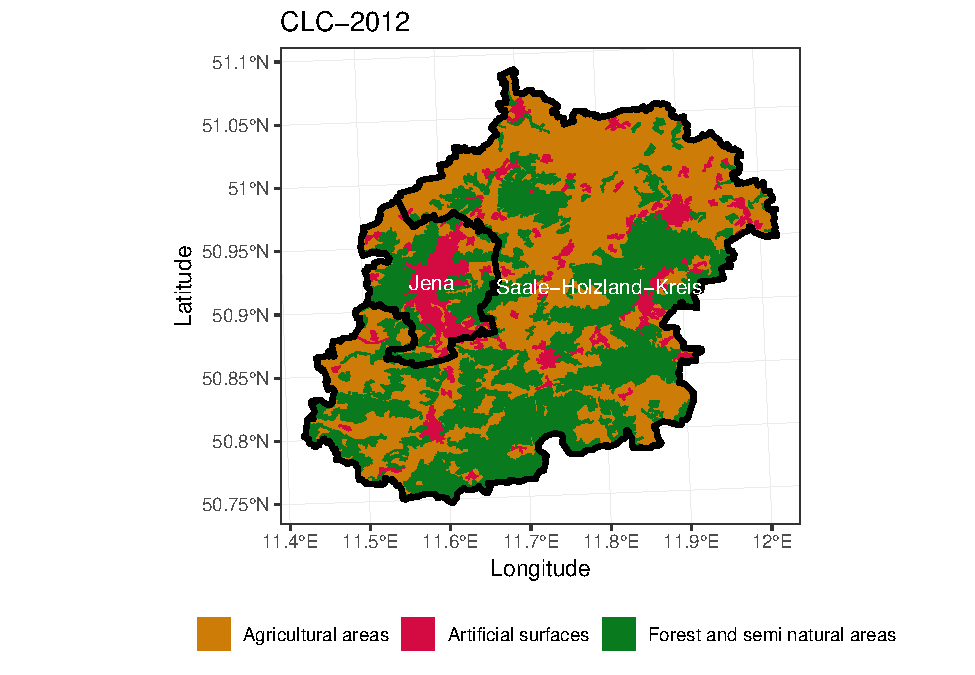
\includegraphics{vignette_files/figure-latex/unnamed-chunk-3-1} 

}

\caption{Overview of study area.}\label{fig:unnamed-chunk-3}
\end{figure}

For ``strange'' or partly invalid geometries, we highly recommend to use
\texttt{GRASS\ GIS}(\textgreater{} 7.6) via the
\href{https://cran.r-project.org/web/packages/rgrass7/index.html}{rgrass7}-package
for the geo-computations. \texttt{GRASS\ GIS} can be easily initialized
via the
\href{https://cran.r-project.org/web/packages/link2GI/index.html}{link2GI}-package:

\begin{Shaded}
\begin{Highlighting}[]

\CommentTok{# If someone wants to use GRASS GIS, one has to installed it first. }
\CommentTok{# Easiest option is via the OSgeo installer. In this example we use GRASS GIS 7.6 }
\CommentTok{# installed on Windows}

\CommentTok{# ... define the installation path (here Windows)}
\NormalTok{my_default_GRASS7 <-}\StringTok{ }\KeywordTok{c}\NormalTok{(}\StringTok{"C:/OSGeo4W64/"}\NormalTok{,}\StringTok{"grass76"}\NormalTok{,}\StringTok{"osgeo4W"}\NormalTok{)}

\CommentTok{# ... define a raster for a GRASS GIS region using }
\CommentTok{#     the administrative boundaries as bounding box}
\NormalTok{r.GRASS <-}\StringTok{ }\NormalTok{raster}\OperatorTok{::}\KeywordTok{extent}\NormalTok{(ADMIN_DIS) }\OperatorTok\StringTok{ }
\StringTok{           }\KeywordTok{raster}\NormalTok{(., }\DataTypeTok{crs =}\NormalTok{ raster}\OperatorTok{::}\KeywordTok{crs}\NormalTok{(ADMIN_DIS))}

\CommentTok{# ... initialisation of GRASS GIS "on the fly"}
\NormalTok{GRASS_INIT <-}\StringTok{ }\NormalTok{link2GI}\OperatorTok{::}\KeywordTok{linkGRASS7}\NormalTok{(}\DataTypeTok{x =}\NormalTok{ r.GRASS, }\DataTypeTok{default_GRASS7 =}\NormalTok{ my_default_GRASS7)}
\end{Highlighting}
\end{Shaded}

\section{3 Calculation of Landscape
Metrics}\label{calculation-of-landscape-metrics}

\subsection{3.1 Effective Mesh Size}\label{effective-mesh-size}

The calculation of the \emph{effective mesh size} is based on
\href{https://doi.org/10.1007/s10980-006-9023-0}{Moser et al. (2007)}.
The indicator gives information on the degree of fragmentation of a
landscape. The result can be interpreted as the probability that two
randomly chosen points in a region will be connected. By multiplying
this probability with the total area of the reporting unit, the result
is converted into an areal unit: the \emph{effective mesh size}
{[}ha{]}. Besides, the indicator is in the meanwhile a well etablished
measurement for landscape fragmentation, and also part of the
\href{https://ec.europa.eu/eurostat/en/web/products-datasets/-/T2020_RN110}{ESMS
Indicator Profile}.

Let's calculate the \emph{effective mesh size} for our two districts!
For the calculation we must define beside a fragmentation geometry
(\texttt{geom.frag}) also either a boundary geometry
(\texttt{geom.boundary}) such as administrative boundaries, or we must
give the total area via \texttt{total.area}.

We can calculate the \emph{effective mesh size} as following:

\begin{Shaded}
\begin{Highlighting}[]
\CommentTok{# CLC 2012}
\NormalTok{TH12.mesh <-}\StringTok{ }\KeywordTok{st_mesh}\NormalTok{(}\DataTypeTok{geom.frag =}\NormalTok{ CLC_}\DecValTok{12} \OperatorTok\StringTok{ }
\StringTok{                                  }\NormalTok{dplyr}\OperatorTok{::}\KeywordTok{filter}\NormalTok{(LABEL1 }\OperatorTok{==}\StringTok{ "Artificial surfaces"}\NormalTok{),}
                     \DataTypeTok{geom.boundary =}\NormalTok{ ADMIN_DIS, }\DataTypeTok{return.geom =} \OtherTok{TRUE}\NormalTok{)}

\CommentTok{# CLC 2018}
\NormalTok{TH18.mesh <-}\StringTok{ }\KeywordTok{st_mesh}\NormalTok{(}\DataTypeTok{geom.frag =}\NormalTok{ CLC_}\DecValTok{18} \OperatorTok\StringTok{ }
\StringTok{                                  }\NormalTok{dplyr}\OperatorTok{::}\KeywordTok{filter}\NormalTok{(LABEL1 }\OperatorTok{==}\StringTok{ "Artificial surfaces"}\NormalTok{),}
                     \DataTypeTok{geom.boundary =}\NormalTok{ ADMIN_DIS, }\DataTypeTok{return.geom =} \OtherTok{TRUE}\NormalTok{)}
\end{Highlighting}
\end{Shaded}

Let's take a look on the results:

\begin{longtable}[]{@{}lrrrr@{}}
\toprule
Name & CLC2012\_CUT & CLC2018\_CUT & CLC2012\_CBC2 &
CLC2018\_CBC2\tabularnewline
\midrule
\endhead
Jena & 814.09006 & 799.63460 & 866.3080 & 851.3873\tabularnewline
Saale-Holzland-Kreis & 13.70294 & 13.68527 & 21.0954 &
21.0122\tabularnewline
\bottomrule
\end{longtable}

Interesting, depending on the measurement the results show a contrary
trend: While the cutting-out (CUT) procedure shows an increasing
landscape fragmentation from 2012 to 2018, the cross-boundary
connections (CBC) procedure shows a decreasing landscape fragmentation.
So take care and choose the appropriate result for your study design!

\subsection{3.2 Urban Sprawl}\label{urban-sprawl}

The \emph{urban sprawl} is defined and calculated according to
\href{https://www.schulthess.com/buchshop/detail/ISBN-9783784340326/Ackermann-Werne-Schweiger-Manue-Sukopp-Ulrich-fuer-Naturschutz-BfN-Bundesam-Editor/Indikatoren-zur-biologischen-Vielfalt?bpmbutton211549=1\&bpmtoken=}{Ackermann
et al. (2013)}. They defined \emph{urban sprawl} as degree of habitat
disturbance by human settlements. The developed so-called
\emph{Freiflächeneffizienz} (FFE, engl. ecological efficiency of open
space) ranges between 0\%, for totally spoiled landscapes, and 100\%,
for areas without any human footprint.

Since the calculation of the \emph{urban sprawl} needs an
\emph{erase}-operation, we will use \texttt{GRASS\ GIS} this time. Let's
start the tool:

\begin{Shaded}
\begin{Highlighting}[]
\CommentTok{# For CLC 2012}
\NormalTok{TH12.urbanSprawl <-}\StringTok{ }\KeywordTok{st_urban_sprawl}\NormalTok{(}\DataTypeTok{tool =} \StringTok{"grass"}\NormalTok{, }
                                    \DataTypeTok{geom.urban =}\NormalTok{ CLC_}\DecValTok{12} \OperatorTok\StringTok{ }
\StringTok{                                     }\NormalTok{dplyr}\OperatorTok{::}\KeywordTok{filter}\NormalTok{(LABEL1 }\OperatorTok{==}\StringTok{ "Artificial surfaces"}\NormalTok{),}
                                    \DataTypeTok{geom.boundary =}\NormalTok{ ADMIN_DIS, }\DataTypeTok{return.geom =} \OtherTok{TRUE}\NormalTok{)}

\CommentTok{# For CLC 2018}
\NormalTok{TH18.urbanSprawl <-}\StringTok{ }\KeywordTok{st_urban_sprawl}\NormalTok{(}\DataTypeTok{tool =} \StringTok{"grass"}\NormalTok{, }
                                    \DataTypeTok{geom.urban =}\NormalTok{ CLC_}\DecValTok{18} \OperatorTok\StringTok{ }
\StringTok{                                     }\NormalTok{dplyr}\OperatorTok{::}\KeywordTok{filter}\NormalTok{(LABEL1 }\OperatorTok{==}\StringTok{ "Artificial surfaces"}\NormalTok{),}
                                    \DataTypeTok{geom.boundary =}\NormalTok{ ADMIN_DIS, }\DataTypeTok{return.geom =} \OtherTok{TRUE}\NormalTok{)}
\end{Highlighting}
\end{Shaded}

Let's take a look on the results:

\begin{longtable}[]{@{}lrr@{}}
\toprule
Name & CLC2012\_FFE & CLC2018\_FFE\tabularnewline
\midrule
\endhead
Jena & 79.31653 & 79.14070\tabularnewline
Saale-Holzland-Kreis & 91.37195 & 91.32509\tabularnewline
\bottomrule
\end{longtable}

The district of Jena has a higher percentage of \emph{urban sprawl}
(79\%) as Saale-Holzland (91\%). Moreover, in both districts the
\emph{urban sprawl} is slightly increasing from 2012 to 2018.

Generally, the calculation of \emph{urban sprawl} is based on grid lines
(fishnet), whose length is transformed (or not) depending on the
intersection with human settlements. Lines between settlements (red) are
more shorten than lines not intersecting any settlements (blue). Lines
intersecting settlements and e.g.~administrative boundaries (green) are
also transformed to account for border effects.

\begin{figure}[!h]

{\centering 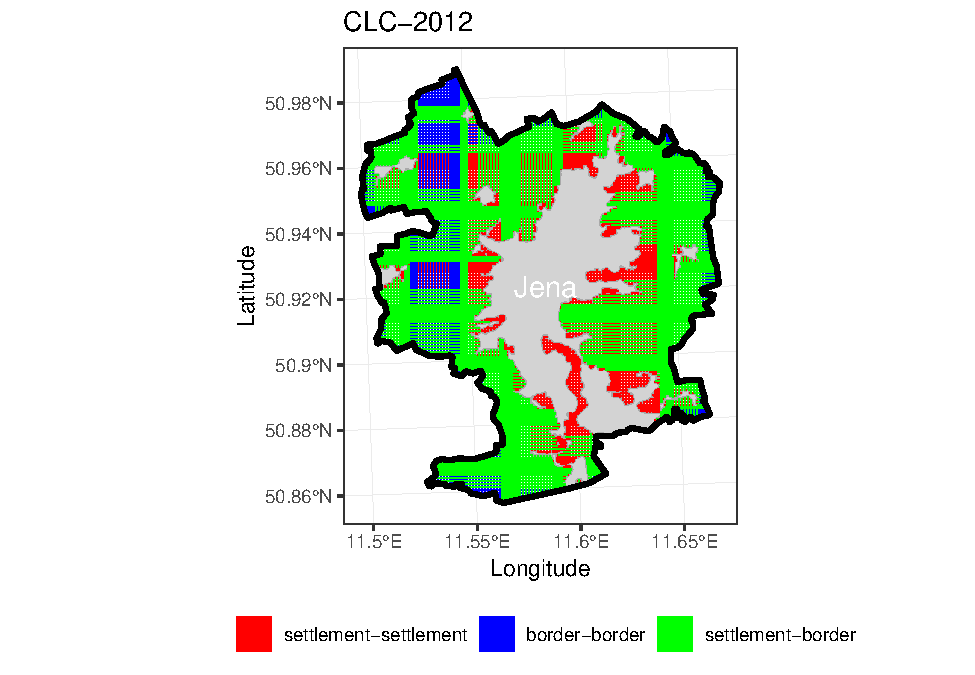
\includegraphics{vignette_files/figure-latex/unnamed-chunk-9-1} 

}

\caption{Urban sprawl of Jena.}\label{fig:unnamed-chunk-9}
\end{figure}

Take care: The result varies depending on the transformation-function
and on the mesh sizes. With a higher mesh size, it is possible to miss
small human settlements resulting in a lower value of \emph{urban
sprawl}.

\subsection{3.3 Integration Index}\label{integration-index}

The \emph{Integration Index} is based on
\href{https://www2.ioer.de/recherche/pdf/2002_meinel_earsel.pdf}{Meinel
\& Winkler (2002)} and gives information on the integration of new
settlement areas into already existing settlement areas. The index
ranges between 0 and 1, and is coarsly categorized as:

\begin{itemize}
\tightlist
\item
  Ratio of 0: Extension without connection to the existing settlement
  area (not integrated)
\item
  Ratio of 0 \textless{}= 1/3: Extension with little connection to the
  existing settlement area (little integrated)
\item
  Ratio of 1/3 \textless{}= 2/3: Rounded off settlement boundaries (well
  integrated)
\item
  Ratio of 2/3 \textless{}= 1: In-fill development in the inner-city
  (fully integrated)
\end{itemize}

If there are geometry problems in the sense that shared boundaries are
not found, the parameter \texttt{dist.new} (e.g.
\texttt{dist.new\ =\ 0.05}) can help to find out of the misery. Again,
to use \texttt{GRASS\ GIS} for processing is recommended but not
necessairy. To get the \emph{integration index} execute:

\begin{Shaded}
\begin{Highlighting}[]
\CommentTok{# For CLC 2018 integration into 2012}
\NormalTok{TH18.integration <-}\StringTok{ }\KeywordTok{st_integration_index}\NormalTok{(}\DataTypeTok{tool =} \StringTok{"grass"}\NormalTok{, }
                        \DataTypeTok{geom.new =}\NormalTok{ CLC_}\DecValTok{18} \OperatorTok\StringTok{ }
\StringTok{                                    }\NormalTok{dplyr}\OperatorTok{::}\KeywordTok{filter}\NormalTok{(LABEL1 }\OperatorTok{==}\StringTok{ "Artificial surfaces"}\NormalTok{), }
                        \DataTypeTok{geom.old =}\NormalTok{ CLC_}\DecValTok{12} \OperatorTok\StringTok{ }
\StringTok{                                    }\NormalTok{dplyr}\OperatorTok{::}\KeywordTok{filter}\NormalTok{(LABEL1 }\OperatorTok{==}\StringTok{ "Artificial surfaces"}\NormalTok{),}
                        \DataTypeTok{geom.boundary =}\NormalTok{ ADMIN_DIS, }\DataTypeTok{return.geom =} \OtherTok{TRUE}\NormalTok{)}
\end{Highlighting}
\end{Shaded}

Let's take a look on the results:

\begin{figure}[!h]

{\centering 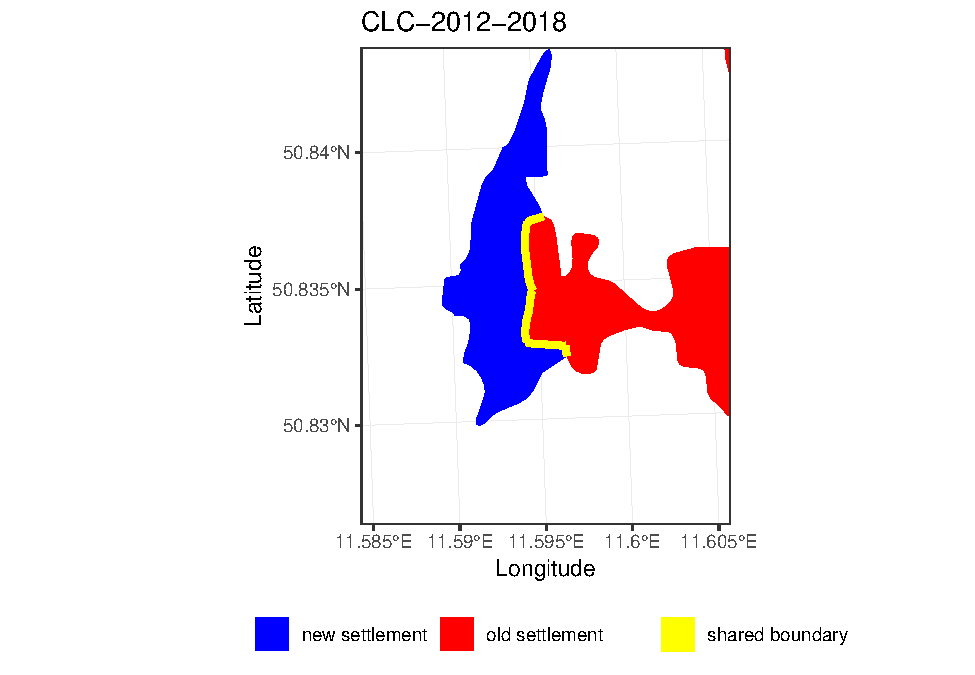
\includegraphics{vignette_files/figure-latex/unnamed-chunk-11-1} 

}

\caption{Integration Index: Shared boundary between old and new settlement.}\label{fig:unnamed-chunk-11}
\end{figure}

\begin{longtable}[]{@{}lr@{}}
\toprule
Name & R\tabularnewline
\midrule
\endhead
Jena & 0.5935216\tabularnewline
Saale-Holzland-Kreis & 0.2532599\tabularnewline
\bottomrule
\end{longtable}

While new settlement areas built between 2012 and 2018 were well
integrated in already existing settlements in the district of Jena
(0.59), the ratio shows only little integration for Saale-Holzland
(0.25).

\subsection{3.4 Shape Indices}\label{shape-indices}

The calculation of the \emph{Shape Indices} is based on
\href{https://link.springer.com/journal/10980}{Forman \& Godron (1986)}.
The index gives information on the compactness of a polygon in
comparison to a circle of the same area. In the context of landscape
metrics we often want to know if a land-use class (e.g.~urban
settlements) is rather compact or frayed. For that we calculate the
(area-weighted) mean shape index (short \emph{MSI}). If a polygon's area
has the form of a circle, the shape index gets the value \texttt{1}.
This simply means that the larger the value, the more frayed the
surface.

Let's take a look on the \emph{MSI} of the urban area of the two
districts:

\begin{Shaded}
\begin{Highlighting}[]
\CommentTok{# MSI for CLC 2012}
\NormalTok{CLC2012.MSI <-}\StringTok{ }\KeywordTok{st_MSI}\NormalTok{(}\DataTypeTok{x =}\NormalTok{ CLC_}\DecValTok{12} \OperatorTok\StringTok{ }\NormalTok{dplyr}\OperatorTok{::}\KeywordTok{filter}\NormalTok{(LABEL1 }\OperatorTok{==}\StringTok{ "Artificial surfaces"}\NormalTok{), }
                      \DataTypeTok{field =} \StringTok{"LABEL1"}\NormalTok{, }\DataTypeTok{geom.boundary =}\NormalTok{ ADMIN_DIS)}

\CommentTok{# MSI for CLC 2018}
\NormalTok{CLC2018.MSI <-}\StringTok{ }\KeywordTok{st_MSI}\NormalTok{(}\DataTypeTok{x =}\NormalTok{ CLC_}\DecValTok{18} \OperatorTok\StringTok{ }\NormalTok{dplyr}\OperatorTok{::}\KeywordTok{filter}\NormalTok{(LABEL1 }\OperatorTok{==}\StringTok{ "Artificial surfaces"}\NormalTok{), }
                      \DataTypeTok{field =} \StringTok{"LABEL1"}\NormalTok{, }\DataTypeTok{geom.boundary =}\NormalTok{ ADMIN_DIS)}
\end{Highlighting}
\end{Shaded}

Let's take a look on the results:

It seems that the district of Jena is slightly more frayed in 2018
(\emph{MSI} of 2.13) compared to 2012 (\emph{MSI} of 2.11), while
Saale-Holzland was getting sliglty more compact (1.99 to 1.97) during
that time.

\subsection{3.5 Edge Length}\label{edge-length}

The importance of \emph{edge length} between land-use classes, e.g.~for
the calculation of ecotones, is based on
\href{http://rosdok.uni-rostock.de/file/rosdok_disshab_0000000980/rosdok_derivate_0000005089/Habilitationsschrift_Walz_2013.pdf}{Walz
(2013)}. Basically, the index gives information on shared edge length
between two land-use classes.

Let's calculate the edge length between \texttt{agricultural\ areas} and
\texttt{forest\ and\ semi\ natural\ areas} in the districts:

\begin{Shaded}
\begin{Highlighting}[]
\CommentTok{# Edge length for CLC 2012}
\NormalTok{TH12.EdgeLength <-}\StringTok{ }\KeywordTok{st_edge_length}\NormalTok{(}\DataTypeTok{x =}\NormalTok{ CLC_}\DecValTok{12} \OperatorTok\StringTok{ }
\StringTok{                                       }\NormalTok{dplyr}\OperatorTok{::}\KeywordTok{filter}\NormalTok{(LABEL1 }\OperatorTok{==}\StringTok{ "Agricultural areas"}\NormalTok{), }
                                  \DataTypeTok{y =}\NormalTok{ CLC_}\DecValTok{12} \OperatorTok\StringTok{ }
\StringTok{                                       }\NormalTok{dplyr}\OperatorTok{::}\KeywordTok{filter}\NormalTok{(LABEL1 }\OperatorTok{==}\StringTok{ "Forest and semi natural areas"}\NormalTok{), }
                                  \DataTypeTok{geom.boundary =}\NormalTok{ ADMIN_DIS, }\DataTypeTok{return.geom =} \OtherTok{TRUE}\NormalTok{)}

\CommentTok{# Edge length for CLC 2018}
\NormalTok{TH18.EdgeLength <-}\StringTok{ }\KeywordTok{st_edge_length}\NormalTok{(}\DataTypeTok{x =}\NormalTok{ CLC_}\DecValTok{18} \OperatorTok\StringTok{ }
\StringTok{                                       }\NormalTok{dplyr}\OperatorTok{::}\KeywordTok{filter}\NormalTok{(LABEL1 }\OperatorTok{==}\StringTok{ "Agricultural areas"}\NormalTok{), }
                                  \DataTypeTok{y =}\NormalTok{ CLC_}\DecValTok{18} \OperatorTok\StringTok{ }
\StringTok{                                      }\NormalTok{dplyr}\OperatorTok{::}\KeywordTok{filter}\NormalTok{(LABEL1 }\OperatorTok{==}\StringTok{ "Forest and semi natural areas"}\NormalTok{), }
                                  \DataTypeTok{geom.boundary =}\NormalTok{ ADMIN_DIS, }\DataTypeTok{return.geom =} \OtherTok{TRUE}\NormalTok{)}
\end{Highlighting}
\end{Shaded}

Now, we have a look on it:

\begin{longtable}[]{@{}lrr@{}}
\toprule
Name & CLC2012\_EdgeLength & CLC2018\_EdgeLength\tabularnewline
\midrule
\endhead
Jena & 98116.8 & 97931.11\tabularnewline
Saale-Holzland-Kreis & 882037.1 & 881234.53\tabularnewline
\bottomrule
\end{longtable}

It is not surprising that the \emph{edge length} {[}m{]} between
\texttt{agricultural\ areas} and
\texttt{forest\ and\ semi\ natural\ areas} is higher in the rural and
larger district of Saale-Holzland. Regarding the change from 2012 to
2018 the \emph{edge length} is slightly decreasing in both districts.
However, the index becomes even more powerful by building appropriate
ratios as \texttt{edge-length\ to\ perimeter\ of\ class\ x}.

\subsection{3.6 Shannon's Diversity
Index}\label{shannons-diversity-index}

The \emph{Shannon's Diversity Index} for landscapes is calculated
according to
\href{https://www.fs.usda.gov/treesearch/pubs/3064}{McGarigal et al.
(1995)}. The index gives information on the diversity of a landscape.
The index is 0 when the area consists only of one land-use class. The
index increases with increasing number of land-use classes or when an
equilibrium of land-use class area is approximated.

The index can be calculated by:

\begin{Shaded}
\begin{Highlighting}[]
\CommentTok{# Shannon's Diversity for CLC 2012}
\NormalTok{TH12.Shannon <-}\StringTok{ }\KeywordTok{st_shannon_index}\NormalTok{(}\DataTypeTok{x =}\NormalTok{ CLC_}\DecValTok{12}\NormalTok{, }\DataTypeTok{field =} \StringTok{"LABEL1"}\NormalTok{, }
                                 \DataTypeTok{geom.boundary =}\NormalTok{ ADMIN_DIS)}

\CommentTok{# Shannon's Diversity for CLC 2018}
\NormalTok{TH18.Shannon <-}\StringTok{ }\KeywordTok{st_shannon_index}\NormalTok{(}\DataTypeTok{x =}\NormalTok{ CLC_}\DecValTok{18}\NormalTok{, }\DataTypeTok{field =} \StringTok{"LABEL1"}\NormalTok{, }
                                 \DataTypeTok{geom.boundary =}\NormalTok{ ADMIN_DIS)}
\end{Highlighting}
\end{Shaded}

Let's take a look on the results:

\begin{longtable}[]{@{}lrr@{}}
\toprule
Name & CLC2012\_Shannon & CLC2018\_Shannon\tabularnewline
\midrule
\endhead
Jena & 1.0910577 & 1.0907722\tabularnewline
Saale-Holzland-Kreis & 0.8526896 & 0.8530465\tabularnewline
\bottomrule
\end{longtable}

The district of Jena has a higher \emph{Shannon Diversity Index} (1.1)
than Saale-Holzland (0.9), and the index is only slightly changing from
2012 to 2018. The higher diversity for Jena is quite surprising, and
appears even contradictory in an ecological sense. This example unveils
directly the weak spots of the index: First, there is no weighting for
ecological valuable land-use classes. For example, an increasing amount
of urban area resulting in a more equitable proportional distribution of
area could increase the index, which, ecologically speaking, is
nonsense. And second, it does not matter if the surfaces are homogeneous
or mosaic-like distributed, the index values stays the same.

\section{4 References}\label{references}

\begin{itemize}
\item
  Ackermann, W., Schweiger, M., Sukopp, U., Fuchs, D., \& Sachteleben,
  J. (2013). Indikatoren zur biologischen vielfalt: Entwicklung und
  bilanzierung {[}Biodiversity indicators. Development and
  accounting{]}. Naturschutz und Biologische Vielfalt, 132.
\item
  Forman, R.T.T.,\& Godron, M. (1986). Landscape Ecology. Cambridge.
\item
  McGarigal, K., \& Marks, B. J. (1995). FRAGSTATS: spatial pattern
  analysis program for quantifying landscape structure. Gen.~Tech.
  Rep.~PNW-GTR-351. Portland, OR: US Department of Agriculture, Forest
  Service, Pacific Northwest Research Station. 122 p, 351.
\item
  Meinel, G., \& Winkler, M. (2002). Spatial analysis of settlement and
  open land trends in urban areas on basis of RS data œ studies of five
  European cities over a 50-year period.
\item
  Moser, B., Jaeger, J. A., Tappeiner, U., Tasser, E., \& Eiselt, B.
  (2007). Modification of the effective mesh size for measuring
  landscape fragmentation to solve the boundary problem. Landscape
  ecology, 22(3), 447-459.
\item
  Siedentop, S., Heiland, S., Lehmann, I., Schauerte-Lüke, N., \&
  HERNIG, A. (2007). Nachhaltigkeitsbarometer Fläche. Regionale
  Schlüsselindikatoren nachhaltiger Flächennutzung für die
  Fortschrittsberichte der Nationalen
  Nachhaltigkeitsstrategie--Flächenziele. Forschungen, 130, 2007.
\item
  Walz, U. (2013). Landschaftsstrukturmaße und Indikatorensysteme zur
  Erfassung und Bewertung des Landschaftswandels und seiner
  Umweltauswirkungen; unter besonderer Berücksichtigung der biologischen
  Vielfalt. Habilitation, Rostock.
\end{itemize}


\end{document}
